\section{Introduction}
\label{sec:intro}

%{\em
%``The goal is to turn data into information, and information into insight.''}
%\vspace{-5pt}
%\begin{flushright}
%--- Carly Fiorina
%\end{flushright}

%Recent interest on geometry processing has been moving towards high-level understanding and intelligent processing of
%three dimensional shapes, with a general goal of discovering patterns about their compositions and structures,
%and relating structures with semantic meanings and functionalities.
%This momentum gives rise to the recent topic of structure-aware geometry processing~\cite{Mitra:2014:SASP}.
%Shape structure implies human knowledge about 3D shapes in terms of part configurations.
%Thus, a natural approach to structural shape analysis and structure-aware shape processing is knowledge-driven,
%where structure is extracted, interpreted and represented with domain-specific knowledge incorporated.
%Examples are like minima-rule-based heuristics for shape segmentation~\cite{Shamir:2008:SMS}, procedural models~\cite{Muller:2006:PMB}
%and rule-based generative models~\cite{Merrell:2011:IFL} for 3D shape modeling.

\rev{As the availability of 3D data increases, due to the developments in both 3D sensing technology as well as 3D modeling software, data-driven approaches become increasingly applicable and useful to 3D shape processing.  In contrast to traditional approaches~\cite{LevyZhang:2011:EGP}, data-driven methods look beyond single objects, instead analyzing sets of shapes jointly to extract meaningful mappings and correlations between them. In addition, these methods are able to learn from data computational models that effectively reason about properties and relationships of shapes without relying on hard-coded rules or explicitly programmed instructions. Leveraging shared information across multiple objects, data-driven methods are able to facilitate high-level shape understanding through discovering geometric and structural patterns among collections of shapes, patterns which serve as strong priors in various geometry processing applications.}

The idea of utilizing data to support geometry processing has been exploited and practiced for many years. However, most existing works based on this idea are confined to the example-based paradigm, mostly leveraging only one core concept of data-driven techniques -- \emph{information transfer}. Typically, the input to these problems includes one or multiple exemplar shapes with some prescribed or precomputed information of interest, and a target shape that needs to be analyzed or processed. These techniques usually establish a \emph{correlation} between the source and the target shapes and transfer the interesting information from the source to the target. The applications of such approaches include a variety of methods in shape analysis (e.g.~\cite{Schaefer:2007:EBS}) and shape synthesis (e.g.~\cite{Merrell:2007:EBM,Ma:2014:ADS}).

As the availability of 3D data increases, several new concepts in data-driven methods are emerging, opening space for new developments in shape analysis and content creation.
\emph{First}, the rich variability of 3D content in existing shape repositories makes it possible to directly reuse the shapes or parts for constructing new 3D models~\cite{Funkhouser:2004:MBE}. \emph{Content reuse} for 3D modeling is perhaps the most straightforward application of big 3D geometric data, providing a promising approach to address the challenging 3D content creation problem.
%
\emph{Second}, high-level shape understanding can benefit from co-analyzing collections of shapes. Several analysis tools demonstrate that shape analysis is more reliable if it is supported by observing certain attributes across a set of semantically related shapes instead of just focusing on a single object. \emph{Co-analysis} requires a critical step of finding correlations between multiple shapes in the input set, which is substantially different from building pair-wise correlation. \rev{A key concept to co-analysis is the \emph{consistency} of the correlations across the entire set, which has both semantic~\cite{Kalogerakis:2010:LMS,Sidi:2011:CS,Wang:2012:ACS} and mathematical~\cite{Huang:2013:SDP} justifications.}
%
\fix{
\emph{Third},
aside from analyzing patterns from a set of shapes,
it is also possible to endorse a subset of the shapes with some semantic information (e.g., part labeling), which can be propogated to the other shapes through learned mappings.
This information propogation evolves the concept of \emph{knowledge transfer} between shapes.
}

\begin{figure}[t!]
\centering
    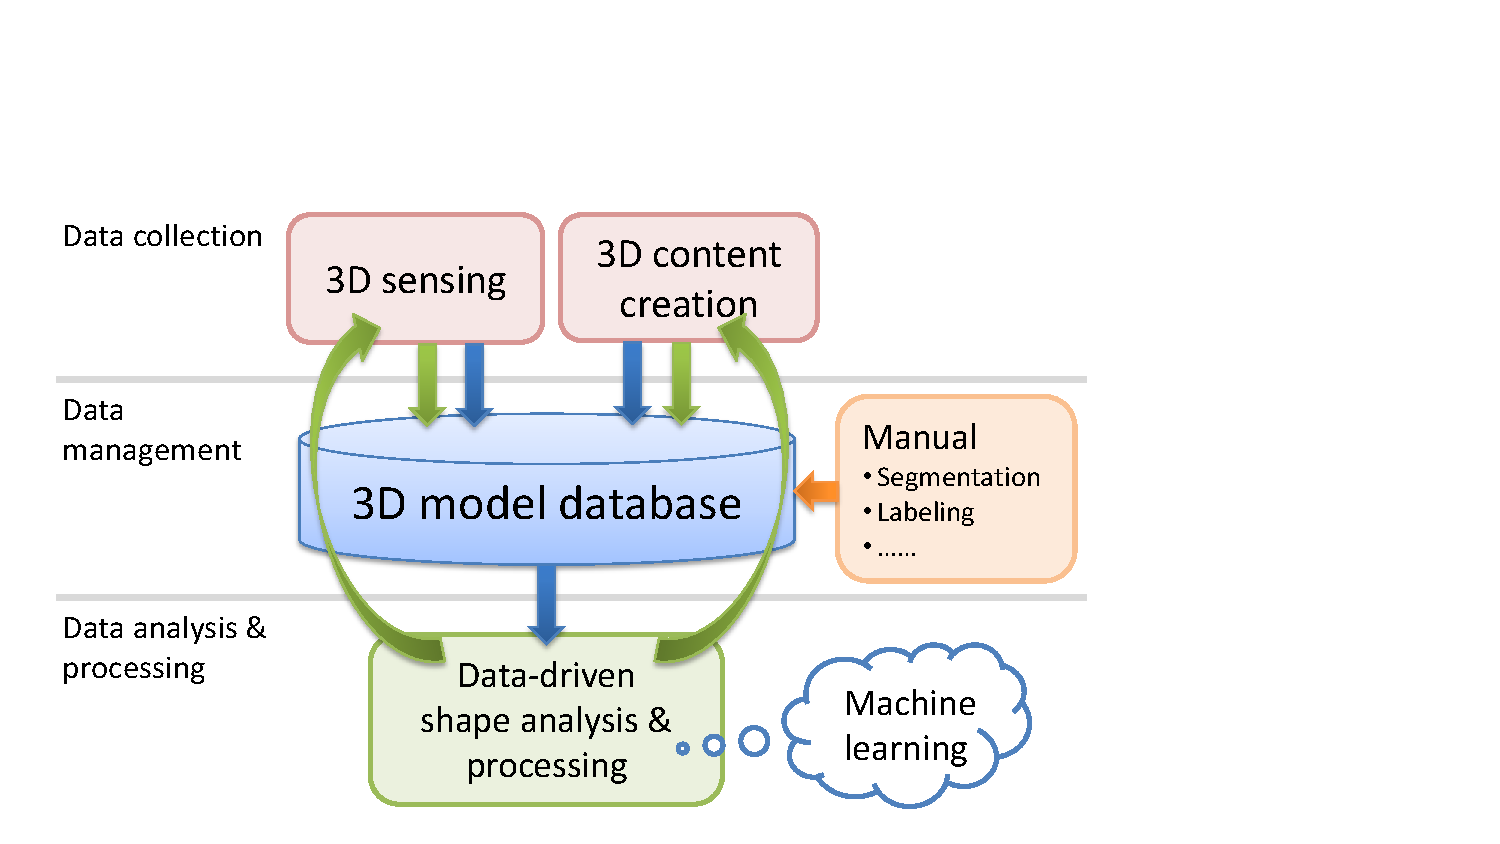
\includegraphics[width=0.99\linewidth]{fig/img/teaser.pdf}
    %\vspace{-.2cm}
    \caption{\rev{Data-driven shape processing and modeling provides a promising solution to the development of ``big 3D data''.
    The two major ways of 3D data generation, 3D sensing and 3D content creation, populate 3D databases with fast growing amount of 3D models.
    The database models are sparsely augmented with manual segmentation and labeling, as well as reasonably
    organized, to support data-driven shape analysis and processing, based on, e.g., machine learning techniques.
    The learned knowledge can in turn support efficient 3D reconstruction and 3D content creation, during which
    the knowledge can be transferred to the newly generated data.
    Such 3D data with semantic information can be included into the database to enrich it and facilitate further data-driven applications.}}
    \label{fig:teaser}
\end{figure}



\paragraph*{Relation to knowledge-driven shape processing.}
Prior to the emergence of data-driven techniques, high-level shape understanding and modeling was usually achieved with knowledge-driven methods.
In the knowledge-driven paradigm, geometric and structural patterns are extracted and interpreted with the help of explicit rules or hand-crafted parameters.
Such examples include heuristics-based shape segmentation~\cite{Shamir:2008:SMS} and procedural shape modeling~\cite{Muller:2006:PMB}.
Although these approaches have certain empirical success, they exhibit several inherent limitations. First, it is extremely difficult to hard-code explicit rules and heuristics that can handle the enormous geometric and structural variability of 3D shapes and scenes in general.
\fix{As a result, knowledge-driven approaches are often hard to generalize well to large and diverse shape collections.}
Another issue is that non-experts find it difficult to interact with knowledge-driven techniques that require as input ``low-level'' geometric parameters or instructions.
%The main problem is that converting human knowledge into hand-crafted rules, heuristics and manually tuned models or algorithms is unlikely to handle the enormous geometric and structural variability of 3D shapes.
%can be used to capture human understanding of 3D shapes.
%Another problem is that human experience and judgment are usually formed with limited observations, which usually does not generalize well to big data.
%This problem becomes especially notable in 3D shapes, among objects that possess significant structural variations.

\rev{In contrast to knowledge driven methods, data-driven techniques learn representations and parameters from data. They usually do not depend on hard-coded prior knowledge, and consequently do not rely on hand-crafted parameters, making these techniques more data-adaptive and thus lead to significantly improved performance in many practical settings.}
The success of data-driven approaches, backed by machine learning techniques, heavily relies on the accessibility of large data collections.
We have witnessed the successful performance improvement of machine learning algorithms by increasing the training set size~\cite{Banko:2001:MPA}. In light of this, the recent developments in 3D modeling tools and acquisition techniques for 3D geometry, as well as availability of large repositories of 3D shapes (e.g., Trimble 3D Warehouse, Yobi3D , etc.), offer great opportunities for developing data-driven approaches for 3D shape analysis and processing.
% and stimulate this direction of research.


\paragraph*{Relation to structure-aware shape processing.}
This report is closely related to the recent survey on ``structure-aware shape processing'' by Mitra and co-workers~\cite{Mitra:2014:SASP},
which concentrates on techniques for structural analysis of 3D shapes, as well as high-level shape processing guided by structure-preservation.
In that survey, shape structure is defined as the arrangement and relations between shape parts, which is analyzed through identifying shape parts, part parameters, and part relations. Each of the three can be determined through manual assignment, predefined model fitting and data-driven learning.

In contrast, our report takes a very different perspective---we focus on how the increasing availability of geometric data has changed the field of shape analysis and processing. In particular, we want to highlight several key distinctions:
\emph{First}, data-driven shape processing goes beyond structure analysis.
For example, leveraging large shape collections may benefit a wider variety of problems in shape understanding and processing, such as parametric modeling of shape space~\cite{Allen:2003:SHB}, hypothesis generation for object and scene understanding~\cite{Zia:2013:DR,Satkin:2012:DDS}, and information transfer between multi-modal data~\cite{Wang:2013:PAS,Su:2014:EID}. Data-driven shape processing may also exploit the data-centered techniques in machine learning such as sparse representation~\cite{Ren:2013:HSC} and feature learning~\cite{Hinton:DBN:2006,Bengio:2009:LDA,Yu:FLI:2010,Krizhevsky:ICDL:2012}, which are not pre-conditioned on any domain-specific or structural prior beyond raw data.
%
\emph{Second}, even within the realm of structure-aware shape processing, data-driven approaches are arguably becoming dominant due to their theoretical and practical advantages, as well as the availability of large shape repositories and recent developments in machine learning.

\begin{figure*}[t!]
\centering
    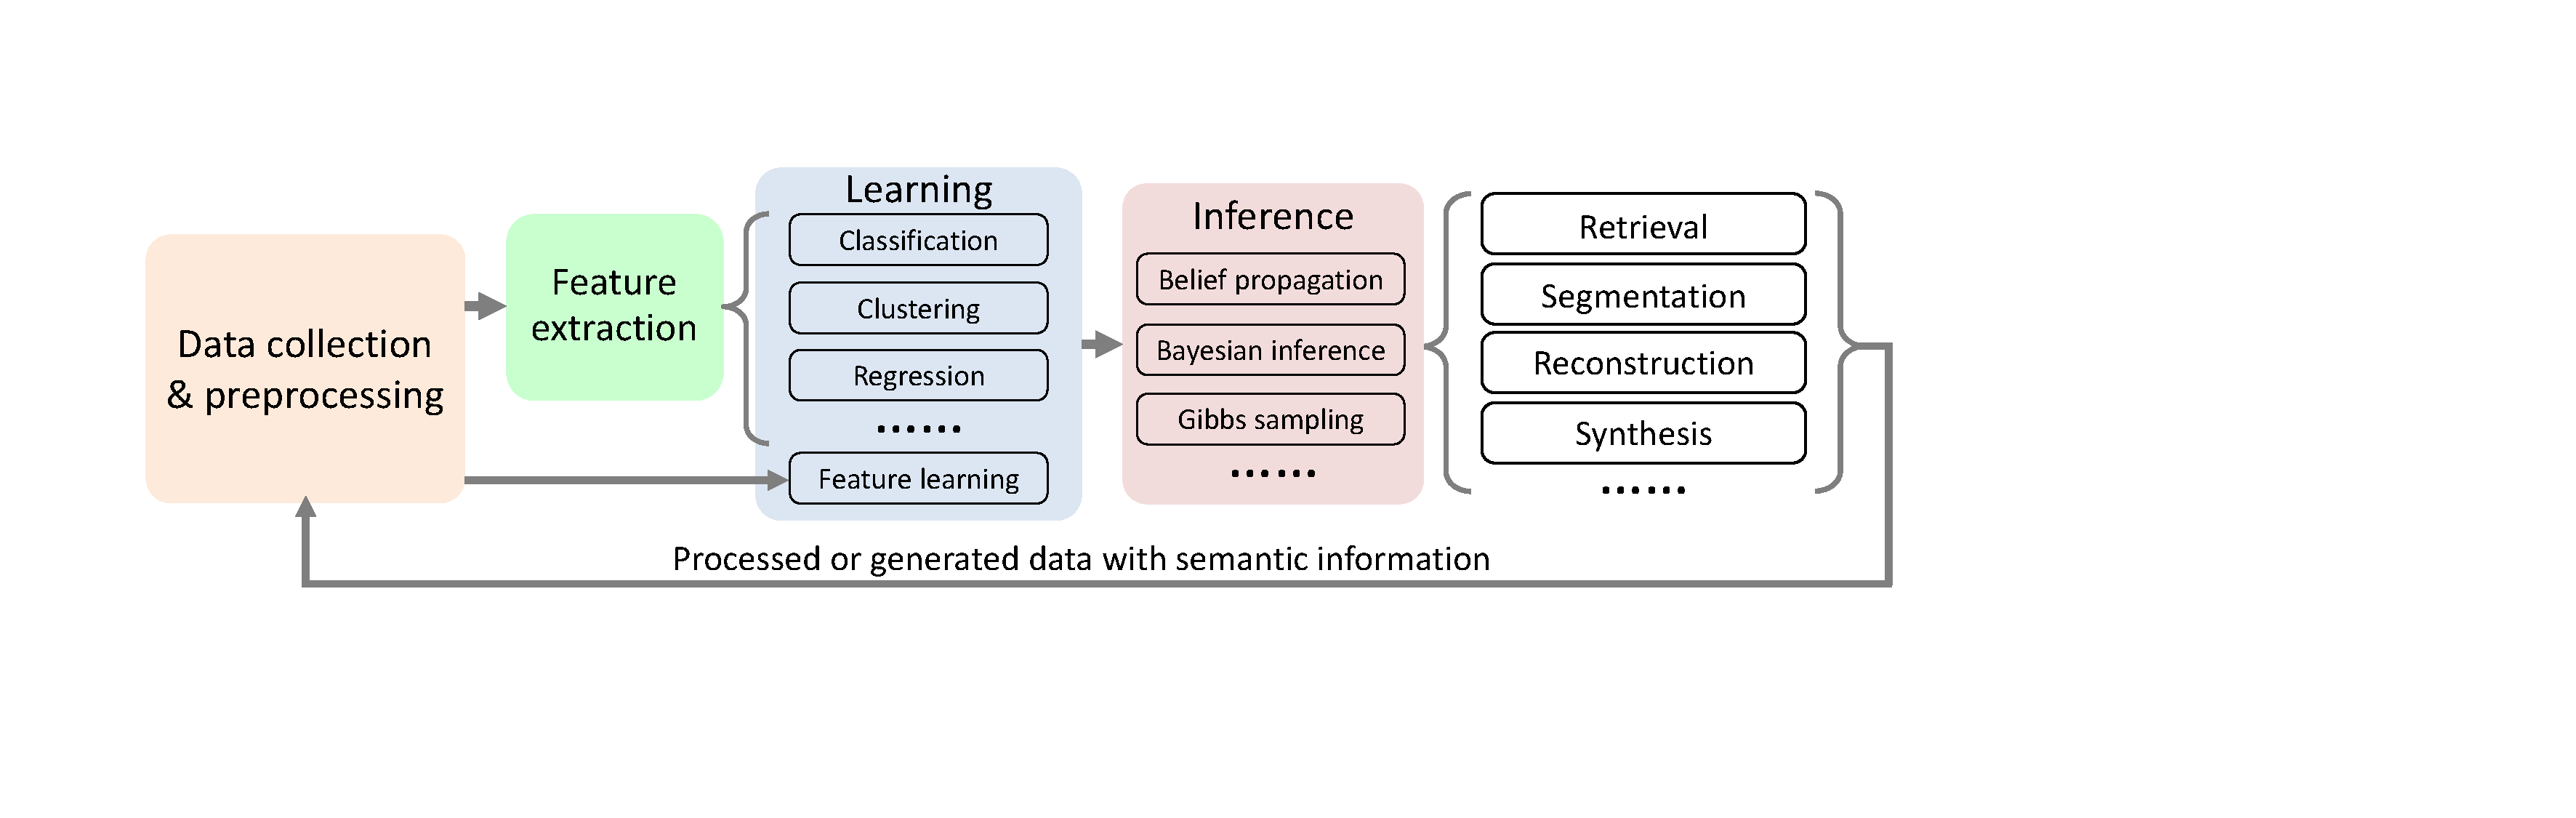
\includegraphics[width=0.9\textwidth]{fig/img/overview.pdf}
    %\vspace{-.4cm}
    \caption{
\rev{The general pipeline of data-driven geometry processing contains four major stages: data collection and preprocessing, feature extraction (or feature learning),
learning and inference. The inference supports many applications which would produce new shapes or scenes through reconstruction modeling or synthesis.
These new data, typically possessing labels for shapes or parts, can be used to enrich the input datasets and enhance the learning tasks in future, forming a data-driven geometry processing loop.}}
    \label{fig:overview}
\end{figure*}



\paragraph*{Vision and motivation.}
\rev{With the emergence of ``big data'', many scientific disciplines have shifted their focus to data-driven techniques. Although 3D geometry data is still far from being as ubiquitous as some other data formats (e.g., photographs), the rapidly growing number of 3D models, the recent developments in fusing 2D and 3D data, and the invention of commodity depth sensors,
%which opens door to low-cost universal acquisition of 3D data associated with 2D images,
have made the era of ``big 3D data'' more promising than ever.}
%The invention of commodity RGB-D camera has opened the door to low-cost, universal acquisition of 3D data, and brought new possibilities for connecting 2D and 3D data. %The connection of 2D and 3D data will provide much more enriched data sources for data-driven methods.
%Furthermore, we expect geometric data to serve as a media that connects multiple modalities.  For example, RGB-D cameras naturally relate images (i.e., the appearance) to shape geometry, or annotated 3D shapes relate geometries to human language.
%
At the same time, we expect data-driven approaches to take one of the leading roles in the reconstruction and understanding of acquired 3D data, as well as the synthesis of new shapes.
%These newly generated data typically comes with rich semantic information produced by data-driven inference, which will enhance exiting shape collections with both reusable content and training labels.
Data-driven geometry processing will close the loop starting from acquisition, analysis, and processing all the way to the generation of 3D shapes (see Figure~\ref{fig:teaser}), and will be a key tool for manipulating big visual data.

Recent years have witnessed a rapid development of data-driven geometry processing algorithms, both in the computer graphics and computer vision communities. Given the research efforts and wide interests in the subject, we believe many researchers would benefit from a comprehensive and systematic survey. \rev{We also hope such a survey can stimulate new theories, problems, and applications.}

\paragraph*{Organization.}
This survey is organized as follows. Section~\ref{sec:overview} gives a high-level overview of data-driven approaches and classifies data-driven methods with respect to their application domains. This section also provides two representative examples for the readers to understand the general work-flow of data-driven geometry processing. The sections following survey the various data-driven shape processing problems in detail, and try to correlate the different methods through comparisons in various aspects. Finally, we conclude our survey by discussing a few key problems involved in designing a data-driven
method for shape processing, listing a set of open challenges in this direction, as well as providing a vision on future research.

\paragraph*{Accompanying online resources.}
In order to assist the reader in learning and leveraging the basic algorithms, we provide an online wikipage~\cite{Wikipage}, which collects tools and source code, together with benchmark data for typical problems and applications of data-driven shape processing. This page will also maintain links and data mining tools for obtaining large data collections of shapes and scenes. This website could serve as a starting point for those who are conducting research in this direction. We also expect it to benefit a wide spectrum of researchers from related fields.


